\subsection{Credit Analysis}

\begin{definition} \hlt{Credit Risk}\\
Risk associated with losses to fixed income investors, due to failure of borrower to make payment of interest or principal. When borrower fails to service their debt, they are in default.
\end{definition}

\subsubsection{Fundamentals of Credit Analysis}

\begin{figure}[H]
\centering
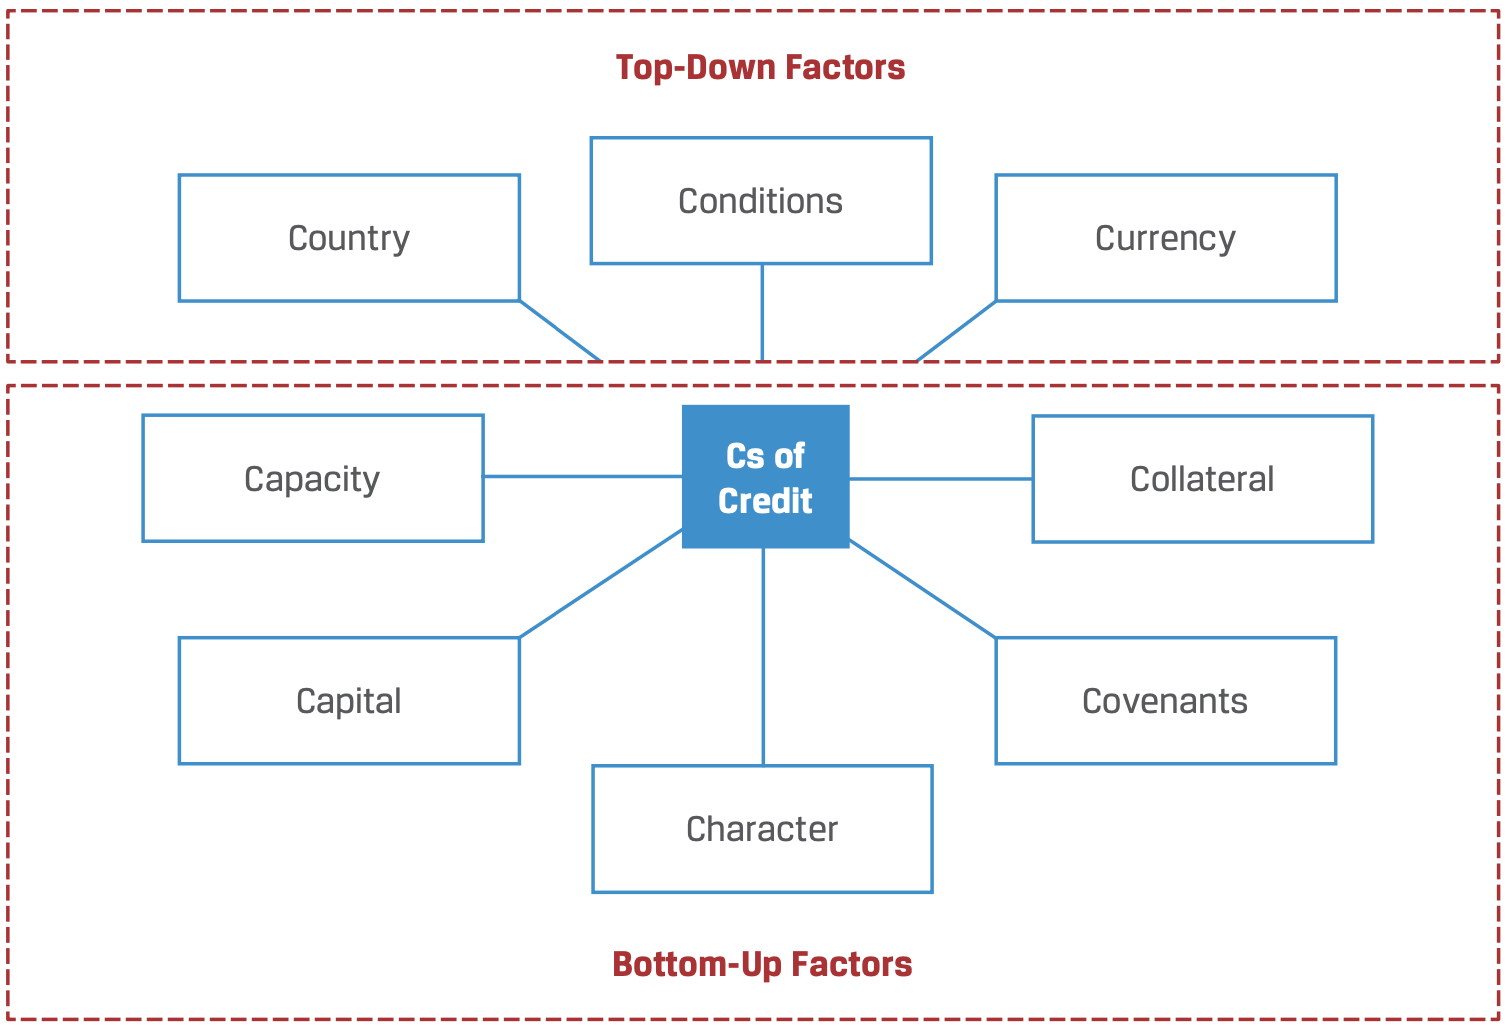
\includegraphics[scale=0.35]{/fi/csofcredit}
\caption{The Cs of Credit Analysis}
\end{figure}

\begin{remark} \hlt{Bottom-Up Credit Analysis Factors}
\begin{enumerate}[label=\roman*.]
\setlength{\itemsep}{0pt}
\item Capacity: measures borrower's ability to make debt payments on time
\item Capital: other resources available to borrower that reduce reliance on debt
\item Collateral: quality and value of assets supporting issuer's indebtedness
\item Covenants: legal terms and conditions the borrowers and lenders agree to as part of bond issue
\item Character: quality of management and willingness of repay indebtedness
\end{enumerate}
\end{remark}

\begin{remark} \hlt{Top-Down Credit Analysis Factors}
\begin{enumerate}[label=\roman*.]
\setlength{\itemsep}{0pt}
\item Conditions: general economic, competitive, and business environment faced by all borrowers that may affect their ability to service or refinance debt
\item Country: geopolitical environment, legal and political system faced by all issuers in a jurisdiction that may affect debt payment
\item Currency: affects issuers whose cash flows are affected by exchange rate changes or who borrow in a currency outside of their jurisdiction, such as sovereign issuers with foreign currency debt.
\end{enumerate}
\end{remark}

\begin{flushleft}
Borrower Types, Sources of Repayment, Sources of Credit Risk
\begin{tabularx}{\textwidth}{p{6.5em}|p{11em}|p{11em}|X}
\hline
\rowcolor{gray!30}
Borrower Type & Primary CF Source & Secondary CF Source & Credit Risk Source \\
\hline
Corporate & 
\xxx Business Operations
\xxx Investment, financing activities
&
\xxx Asset sales
\xxx Divestitures
\xxx Additional debt issuance
\xxx Equity issuance
&
\xxx Economic contraction
\xxx Strategic shifts in business and market environment
\xxx Increase competition
\xxx Reduced pricing power
\xxx Shrinking operating margin, increased losses
\xxx Excessive debt service needs \\
\hline
Soverigen or Public Entity & 
\xxx Taxes (income, sales, VAT, capital gains, wealth-based)
\xxx Tariffs, fees, other government revenue
&
\xxx Newly issued debt
\xxx Sale of public assets, privatisation
&
\xxx Economic contraction
\xxx Political uncertainty
\xxx Excessive debt service needs
\xxx Expansionary economic policies
\xxx Budget deficits
\xxx Tax cuts
\xxx Limited ability to collect taxes \\
\hline
\end{tabularx}
\end{flushleft}

\begin{figure}[H]
\centering
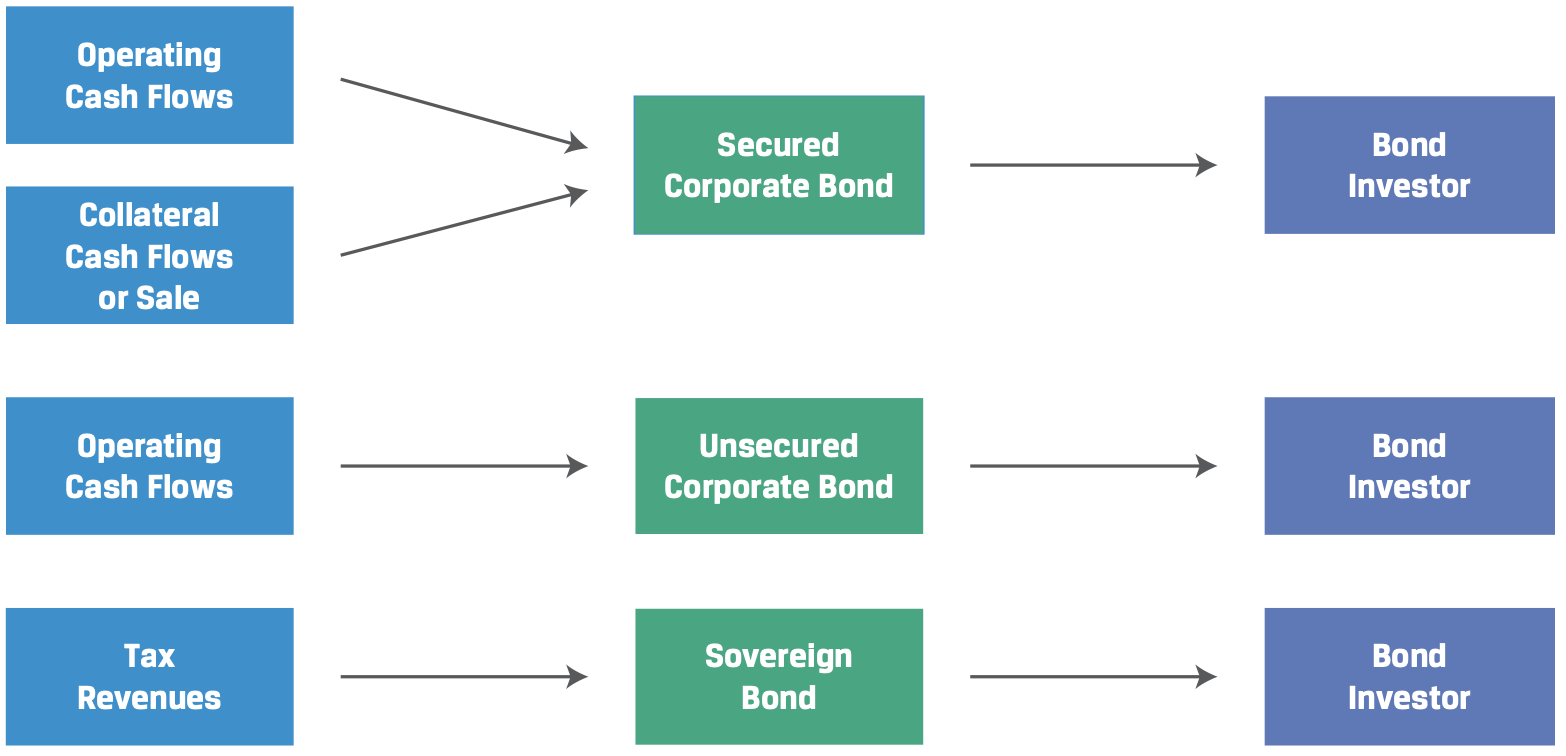
\includegraphics[scale=0.35]{/fi/sovcorpsourceofpayment}
\caption{Sovereign and Corporate Bond Sources of Repayment}
\end{figure}

\begin{remark} \hlt{Illiquid vs Insolvent}\\
Illiquid issuer is an issuer unable to raise cash to service debt.\\
Insolvent issuer has assets falling below the value of its debt.\\
An illiquid issuer may not necessarily be insolvent, but could still default.
\end{remark}

\begin{remark} \hlt{Bond Identure Clauses}
\begin{enumerate}[label=\roman*.]
\setlength{\itemsep}{0pt}
\item Cross-Default Clause: a default on one bond issuer causes a default on all issues
\item Pari Passu Clause: all bonds of certain type rank equally in the default process
\end{enumerate}
If both provisions exist on unsecured debt, a default on one issuer implies all holders of unsecured claims have access to general assets of the issuer to satisfy their obligations.\\
If both provisions exist on secured debt, default on any obligation of the issuer will grant access to general assets of the company and to assets pledged as collateral for the debt.\\
If value of pledged assets fall below amount of pari passu secured debt, secured bond investor have credit losses.
\end{remark}

\begin{remark} \hlt{Components of Credit Risk}
\begin{enumerate}[label=\roman*.]
\setlength{\itemsep}{0pt}
\item Probability of Default (POD): likelihood that issuer fails to make full and timely payments of principal and interest. Measure is typically annualised.
\item Loss Given Default (LGD): investor's loss conditional on issuer event of default. Combines severity of loss under fault scenario with amount of investor's claim at time of default.
\item Recovery Rate (RR): percentage of outstanding debt claim recovered when issuer defaults.
\item Loss Severity ($1 - \text{RR}$): unrecovered portion of the claim
\item Expected Exposure (EE) or Exposure at Default (EAD): amount an investor may expect to lose in case of default, equal to loan or bond face value plus accrued interest, less current market value of collateral.
\end{enumerate}
\begin{align}
\text{Expected Loss EL} &= \text{POD} \times \text{LGD} \nonumber \\
\text{LGD} &= \text{EE} \times (1 - \text{RR}) \nonumber
\end{align}
Using annualised EE as estimate of annualised credit spread over risk-free benchmark for credit risk,
\begin{equation}
\text{Credit Spread} \approx \text{POD} \times \text{LGD} \nonumber
\end{equation}
If actual credit spread of issue is higher than this estimated credit spread, investor is more than fairly compensated for the credit risk of the investment. 
\end{remark}

\begin{figure}[H]
\centering
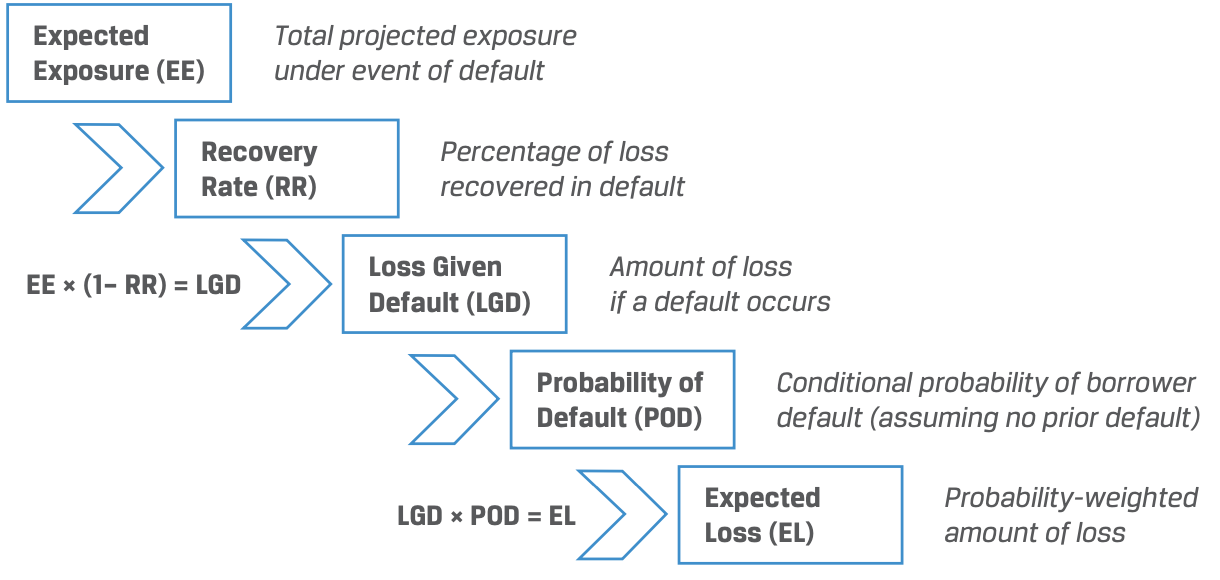
\includegraphics[scale=0.4]{/fi/creditriskcomp}
\caption{Components of Credit Risk}
\end{figure}

\begin{remark} \hlt{Drivers of Probability of Default}
\begin{enumerate}[label=\roman*.]
\setlength{\itemsep}{0pt}
\item Profitability: stable, predictable cash flows and profits. Higher is better.
\item Coverage: sufficient cash flows/profits to make debt payments. Higher is better.
\item Leverage: relative reliance on debt financing. Lower is better.
\end{enumerate}
\end{remark}

\begin{figure}[H]
\centering
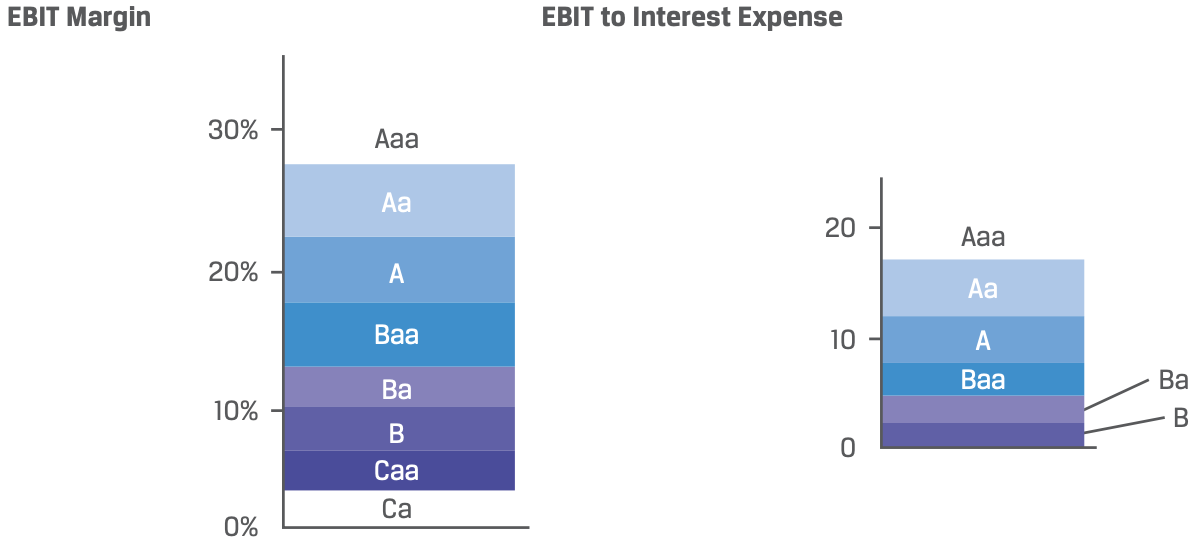
\includegraphics[scale=0.38]{/fi/keyfinratiocredit1}
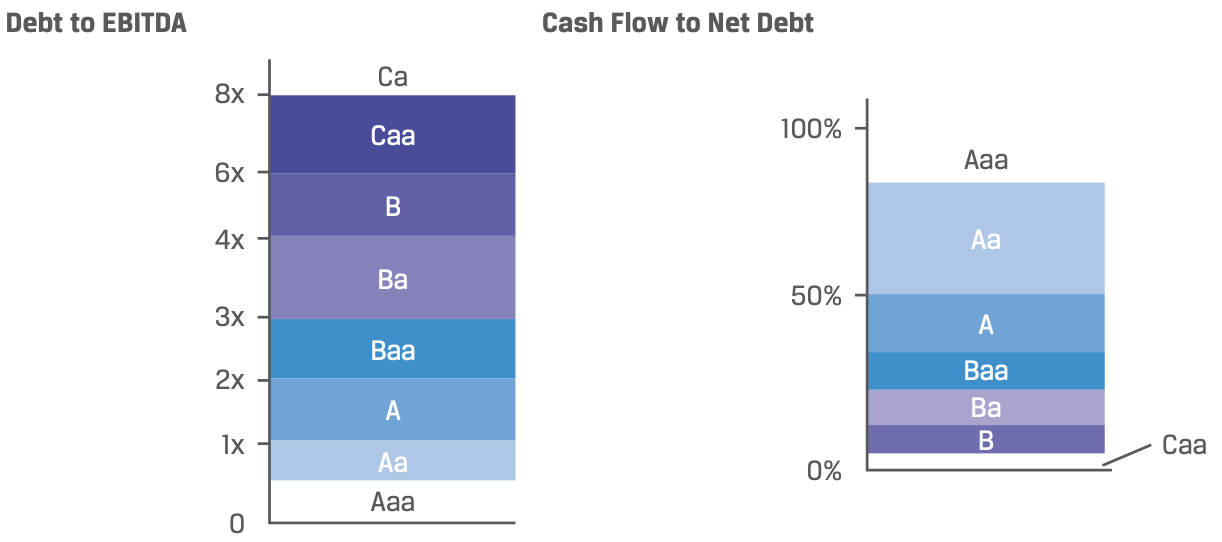
\includegraphics[scale=0.38]{/fi/keyfinratiocredit2}
\caption{Key financial ratios for corporate credit risk and ratings}
\end{figure}

\begin{remark} \hlt{Drivers of Loss Given Default}\\
A function of nature and seniority of creditor's claim in a default scenario.\\
More senior, secured debt will have lower losses given default than junior, unsecured debt.\\
High-yield issuer may issue secured debt with secondary source of repayment in event of default. Hence high-yield debt can have lower loss given default than unsecured bonds of investment grade issuer.\\
Greatest risk in unsecured investment grade debt is an increase in probability of default due to deterioration of issuer's financial situation.
\end{remark}

\begin{definition} \hlt{Hazard Rate (HR)}\\
Conditional probability of default given that default has previously not occured.
\end{definition}

\begin{definition} \hlt{Probability of Survival (POS)}\\
Assuming a constant hazard rate, at time $t$, 
\begin{align}
\text{POS}_t &= 1 - \text{Cumulative POD} \nonumber \\
&= (1-\text{HR})^t \nonumber \\
\text{POD}_t &= \text{HR} \times \text{POS}_{t-1} \nonumber
\end{align}
Note that POS decreases over time, and POD depends on POS from prior period.\\
In first year, POD $=$ HR, as PS $=1$ at inception. In subsequent periods, PD $<$ HR.
\end{definition}

\begin{definition} \hlt{Credit Valuation Adjustment (CVA)}\\
Sum of present value of expected loss for each period. CVA is monetary value of credit risk in present value terms; it is difference in value of risk-free bond and identical risky bond.\\
Use of actual default rate may overstate observed value of bond as it does not include default risk premium associated with timing uncertainty of possible defaults.
\begin{equation}
\text{CVA} = \text{Price of Risk-Free Bond} - \text{Price of Risky Bond} = \text{Sum of PV of Expected Loss}\nonumber
\end{equation}
\end{definition}

\begin{remark} \hlt{Risk Neutral Probability of Default}\\
Probability of default implied on current market price. Solve for POD below:
\begin{equation}
\text{Market Price of Bond} = \frac{\text{EE} \times (1-\text{POD}) + (1- \text{LGD})\times \text{POD}}{1 + \text{Benchmark Rate}} \nonumber
\end{equation}
The implied RR may also be derived from the equation, given POD.\\
If POD assumed is greater than the risk-neutral POD, then implied RR will be higher.\\
Given the market price and credit spread, risk neutral POD and RR are positive correlated.\\
Note that in the model, POD an RR are both estimates.
\end{remark}

\begin{remark} \hlt{ESG Considerations for Credit Risk}\\
Estimated POD and LGD to account for ESG-related risk exposure.\\
Climate and green bonds are issued with proceeds earmarked for environmental purposes, and may come with tax incentives to enhance attractiveness to investors.\\
Catastrophe and pandemic bonds resemble an insurance product, offering high interest payments in return for takin on risk of losing capital should a pandemic occur.
\end{remark}

\subsubsection{Credit Scores, Ratings, and Spreads}

\begin{remark} \hlt{Uses of Credit Ratings}
\begin{enumerate}[label=\roman*.]
\setlength{\itemsep}{0pt}
\item Comparing credit risk of issuers across industries and bond types, assessing changing credit conditions
\item Assessing credit migration risk (risk that credit rating downgrade will decrease value of bonds and potentially trigger other contractual clauses)
\item Meeting regulatory, statutory, or contractual requiremeents
\end{enumerate}
\end{remark}

\begin{flushleft}
Long-Term Rating Matrix, Investment Grade vs Non-Investment Grade
\begin{tabularx}{\textwidth}{p{9em}|p{8em}|X|X|X}
\hline
\rowcolor{gray!30}
Grade & Detail & Moody's & S\&P & Fitch \\
\hline
Investment & High-Quality & Aaa & AAA & AAA \\
& & Aa1 & AA+ & AA+ \\
& & Aa2 & AA & AA \\
& & Aa3 & AA- & AA- \\
& Upper-Medium & A1 & A+ & A+ \\
& & A2 & A & A \\
& & A3 & A- & A- \\
& Low-Medium & Baa1 & BBB+ & BBB+ \\
& & Baa2 & BBB & BBB \\
& & Baa3 & BBB- & BBB- \\
\hline
Non-Investment & Low, Speculative & Ba1 & BB+ & BB+ \\
(Junk, High-Yield) & & Ba2 & BB & BB \\
& & Ba3 & BB- & BB- \\
& & B1 & B+ & B+ \\
& & B2 & B & B \\
& & B3 & B- & B- \\
& & Caa1 & CCC+ & \\
& & Caa2 & CCC & CCC \\
& & Caa3 & CCC- & \\
& & Ca & CC & CC \\
& & Ca & C & C \\
& Default & C & D & D \\
\hline
\end{tabularx}
\end{flushleft}
Rating agencies also provide an outlook (positive, negative, stable).\\
Higher rated bonds trade at lower spreads relative to benchmark rates.

\begin{remark} \hlt{Limitations of Credit Ratings from Agencies}
\begin{enumerate}[label=\roman*.]
\setlength{\itemsep}{0pt}
\item Credit ratings lag market pricing. Two bonds with same rating may trade at different yields as credit ratings focus on expected loss, but market pricing for distressed debt focuses more on default timing and expected recoveries.
\item Risks such as litigation, natural disasters, environmental risks, acquisitions and equity buybacks using debt are not easily predicted or captured in credit ratings. Agencies may take different views on likelihood of such events, leading to split ratings.
\item Mistakes may occur; corporate fraud may lead to companies with high credit ratings suddenly defaulting.
\end{enumerate}
\end{remark}

\begin{remark} \hlt{FICO Score Factors}
\begin{enumerate}[label=\roman*.]
\setlength{\itemsep}{0pt}
\item $35\%$ Payment History: presence or lack of such information such as delinquency, bankruptcy, court judgments, repossessions, foreclosures
\item $30\%$ Debt Burden: credit card debt-to-limit ratios, $\#$ accounts with balances $>0$, total amount owed
\item $15\%$ Length of Credit History: average age of accounts on credit file, age of oldest account
\item $10\%$ Types of Credit Used: use of instalment payments, consumer finance, mortgages
\item $10\%$ Recent Searches for Credit: 'hard' credit inquiries when consumers apply for new loans
\end{enumerate}
\end{remark}

\begin{definition} \hlt{Credit Migration}\\
A change in rating reflects a change in bond's credit risk.\\
Change in price of the bond depends on modified duration of the bond, and change in spread resulting from change in credit risk as reflected by the credit migration.
\begin{equation}
\Delta \% \text{PV}^{\text{Full}} = - \text{AnnModDur} \times (\Delta \text{Spread}) + \frac{1}{2} \text{AnnConvexity}(\Delta \text{Spread})^2 \nonumber
\end{equation}
\end{definition}

\begin{definition} \hlt{Credit Spread Risk}\\
Risk that yield spreads widen due to deteriorating conditions, causing credit-risky bond prices to increase.\\
Credit spread risk arises from macroeconomic, issuer-specific, market related factors.
\end{definition}

\begin{remark} \hlt{Credit Spread Risk Macroeconomic Factors}\\
Credit risk changes are largely in line with the economic cycle, where strong growth and high profits reduces POD and thus causing spreads to contract. In recession, POD increases, causing spreads to widen.
\end{remark}

\begin{figure}[H]
\centering
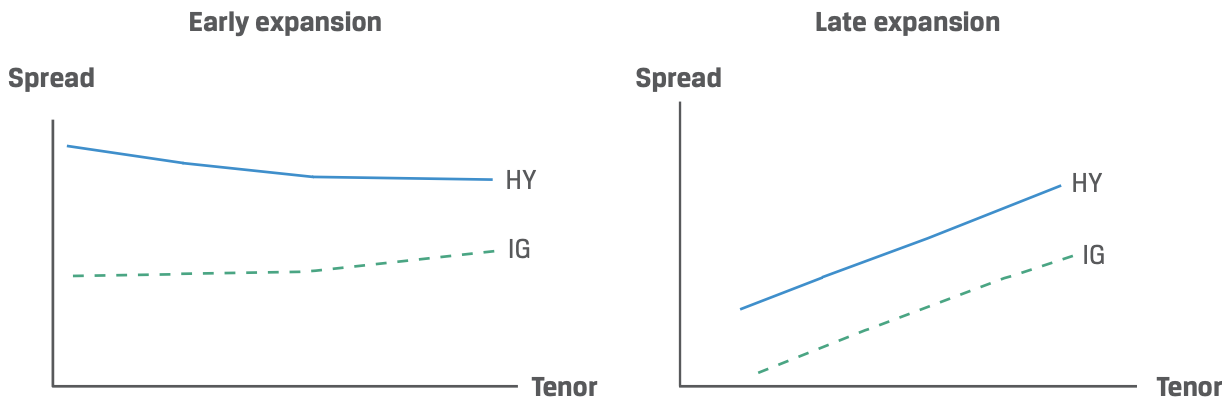
\includegraphics[scale=0.38]{/fi/creditspreadeconcycle1}
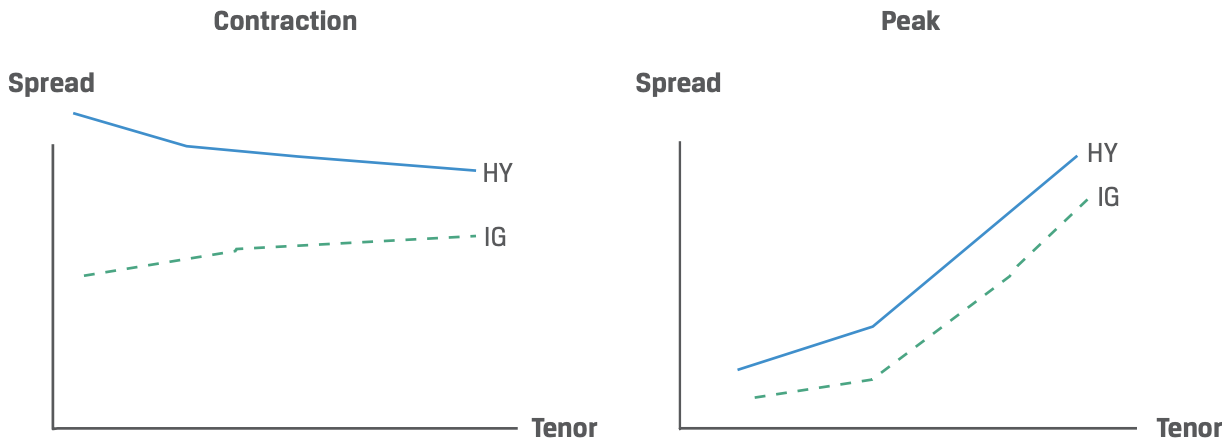
\includegraphics[scale=0.38]{/fi/creditspreadeconcycle2}
\caption{Credit spreads over the economic cycle}
\end{figure}

\begin{remark} \hlt{Credit Spreads Behaviours of Issuers}
\begin{enumerate}[label=\roman*.]
\setlength{\itemsep}{0pt}
\item Investment grade issuers have lower yield spreads than high-yield issuers due to lower expected loss
\item Yield spreads increase with maturity as POD increases over longer time frames, giving rise to upward-sloping credit spread curves (when plotting credit spread vs tenor).
\begin{enumerate}[label=\roman*.]
\setlength{\itemsep}{0pt}
\item In economic recessions, high-yield and investment grade curves rise and flatten as probability of near-term default increases. High-yield curve may invert in this stage of economic cycle.
\item In economic expansions, high-yield and investment grade curves fall and steepen as probability of near-term default decreases. Credit curves will be lowest and most steep at peak of curve.
\end{enumerate}
\item Across issuers, dispersion of yield spreads for high-yield issuers is higher than for investment-grade issuers
\item High-yield spreads fluctuate more than investment grade spreads as economic conditions change. High-yield spreads can widen dramatically in times of crisis as investors sell riskier assets and buy safer assets in a flight to quality. High-yield issues tend to be less liquid, hence bid-offer spreads may widen more than for investment grade issues in recession.
\end{enumerate}
\end{remark}

\begin{remark} \hlt{Incentives for Exposure to Higher Credit Spread Risk}
\begin{enumerate}[label=\roman*.]
\setlength{\itemsep}{0pt}
\item Diversification: high-yield bond prices have low/negative correlation with investment grade bonds, hence may diversify a fixed-income portfolio
\item Capital Appreciation: larger spread changes for high-yield issues produce larger price gains during economic recoveries compared to investment grade issues.
\item Equity-Like Returns: high-yield debt offers equity-like returns with lower volatility than equity markets
\end{enumerate}
\end{remark}

\begin{remark} \hlt{Drivers of Higher Credit Yield Spreads}
\begin{enumerate}[label=\roman*.]
\setlength{\itemsep}{0pt}
\item Increasing regulations of broker-dealers and market makers in corporate bonds have increased the cost of funding bond positions
\item Funding stresses in markets may increase risk aversion
\item Heavy new issuance of debt into bond markets might not be met by increased demand
\end{enumerate}
\end{remark}

\begin{remark} \hlt{Issuer-Specific Factors on Credit Yield Spread}\\
Financial performance of issuer will have significant impact on yield spread level and volatility. An issuer with problems servicing its debt will have wider yield spreads than average for their credit rating.
\end{remark}

\begin{remark} \hlt{Market Liquidity Risk}\\
Transaction costs of trading a bond. May be assessed through analysing the bid-offer spreads of market makers. Wider bid-ask spread implies higher costs of trading, and hence higher market liquidity risk.\\
Issuers with more debt outstanding or with higher credit ratings have more actively traded bonds, hence has narrower bid-ask spreads and lower market liquidity risk.\\
Bid-ask spreads may widen substantially for high-yield issuers during financial stress, and market liquidity falls dramatically, increasing risk aversion, causing wider bid-ask spreads to spill over to investment grade issuers.\\
Bd-ask spreads of market makers may be used to isolate the component of the yield spread that is due to liquidity risk. The difference in yield of bid and ask prices is compensation for liquidity risk.
\end{remark}

\begin{remark} \hlt{XVA} \\
XVA is an adjustment that comprises the observed spread between corporate and benchmark bond yields.\\
These adjustments includes CVA, funding valuation adjustment (FVA), liquidity valuation adjustment (LVA), taxation valuation adjustment (TVA).
\end{remark}

\begin{remark} \hlt{Changes in Credit Spread}\\
Due to changes in investor perceptions about future probability of default and recovery rates change. Perceptions depend on expectations about the state of economy. Expectations of impending recessions may lead to higher defaults and lower recovery rates.
\end{remark}

\begin{definition} \hlt{Term Structure of Credit Spreads}\\
Relationship between credit spreads and maturity. Term structure is useful gauge for issuers, underwriters, and investors in measuring risk-return trade-off for bonds across ratings and/or sectors across maturities. Term structure is also used for pricing a new issue, and determining relative valuation of an existing issue.
\end{definition}

\begin{figure}[H]
\centering
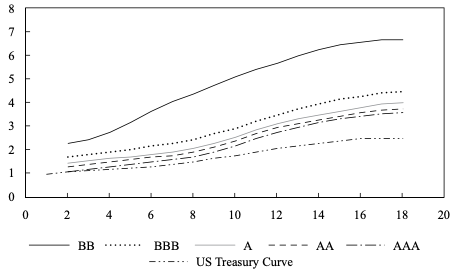
\includegraphics[scale=0.5]{/fi/totalyields}
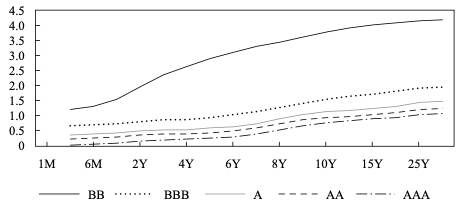
\includegraphics[scale=0.5]{/fi/spreads}
\caption{Total yields and credit spread curve}
\end{figure}

\begin{remark} \hlt{Creation of Spread Curve}
Credit spread is inversely related to recovery rate and positively related to probability of default. If interpolation cannot be used due to availability of data, or when benchmark bonds are thinly traded,  spread relative to a swap fixed rate (corresponding to maturity of bond) may be used.\\
To create spread curve, the bonds used should have similar credit characteristic.\\
Differences in seniority, first/second lien provisions, embedded options may distort the computed credit spread.
\end{remark}

\begin{remark} \hlt{Determinants of Shape of Credit Spread Curve}\\
Expectations on future recovery rates and default probabilities. If default probabilities are expected to be higher, or recovery rates lower in the future, credit curve will be positively sloped.\\
Flat credit curves indicate stable expectations over time.
\end{remark}

\begin{remark} \hlt{Determinants of Term Structure of Credit Spreads}
\begin{enumerate}[label=\roman*.]
\setlength{\itemsep}{0pt}
\item Credit quality: high quality issue term structures are flat or slightly upward sloping. Lower-rated issues have steeper spread curves, reflecting greater uncertainty and greater sensitivity to business cycle.
\item Financial conditions: spreads narrow in expansions and widen in recessions. Benchmark yields are higher while credit spreads are narrower during expansions.
\item Market demand and supply: less liquid maturities will have higher spreads. Higher liquidity issues will influence the credit curves more. As newly issued bonds are more liquid, when issuer refinances, the spread may narrow for longer maturity, possibly leading to an inverted credit spread curve.
\item Equity market volatility: increase in equity volatility will widen spreads and influence shape of credit spread curve, as structural models use stock price volatility and balance sheet structure for POD.
\end{enumerate}
\end{remark}

\begin{remark} \hlt{Factors of Securitised Debt Credit Analysis}
\begin{enumerate}[label=\roman*.]
\setlength{\itemsep}{0pt}
\item Collateral Pool: homogeneity of pool refers to similarity of assets within the pool. Granularity refers to transparency of assets within the pool. Highly granular pol may have hundreds of underlying assets; portfolio summary statistics may be used.
\item Servicer Quality: investor may face operational and counterparty risk of the servicer. The servicer's past history is an indication of servicer quality.
\item Structure: tranching and other management of credit and other risks in a collateral pool.
\end{enumerate}
\end{remark}

\begin{flushleft}
Summary of asset types and characteristics of core structured finance asset classes
\begin{tabularx}{\textwidth}{p{8.4em}|p{11em}|p{6em}|p{5em}|p{6em}|p{7.5em}}
\hline
\rowcolor{gray!30}
Deal & Collateral & Risk Horizon & Granularity & Homogeneity & Approach \\
\hline
Asset-Backed CP & Commercial discount credits or credit advances & Short-term & Granular & Homogeneous & Book \\
\hline
Auto ABS & Auto loans or leases & Medium-term & Granular & Homogeneous & Portfolio \\
\hline
CMBS & Commercial mortgages & Long-term & Non-gran. & Heterogeneous & Loan by Loan \\
\hline
Consumer ABS & Consumer loans & Medium-term & Granular & Homogeneous & Portfolio \\
\hline
CRE Loans & Commercial RE loans & Long-term & Non-gran. & Heterogeneous & Loan by loan \\
\hline
Credit Cards & Credit card balances & Short-term & Granular & Homogeneous & Book \\
\hline
Credit-linked notes & Any financial assets & Medium-term & Single asset & N.A. & Asset by asset$^{(1)}$ \\
\hline
LL CLOs & Leveraged corp loans & Medium-term & Non-gran. & Heterogeneous & Loan by loan \\
\hline
PF CLOs & Project finance debt & Long-term & Non-gran. & Heterogeneous & Loan by loan \\
\hline
RMBS & Residential mortgages & Long-term & Granular & Homogeneous & Portfolio$^{(2)}$ \\
\hline
SME ABS & Loans to SMEs & Medium-term & Granular & Mixed & Portfolio$^{(2)}$ \\
\hline
Trade receivables & Commercial credit & Short-term & Granular & Homogeneous & Book \\
\hline
\end{tabularx}
$^{(1)}$ May also use pass-through rating\\
$^{(2)}$ May also use loan-by-loan
\end{flushleft}

\subsubsection{Structural and Reduced Form Models of Credit Risk}

\begin{remark} \hlt{Structural Credit Models}\\
Aim to explain why default occurs. Default intensity estimated on company financial statement ratios and variables, and macroeconomic variables. Model depends on structure of company's balance sheet, and the key variable is asset value. Asset value has a probability distribution, with a portion below the default barrier. \\
The default probability increases with variance of future asset value, with greater time to $T$, and greater financial leverage. Less leverage reduces the default barrier and hence reduces the POD. These factors indicate that credit risk is linked to option pricing theory.
\end{remark}

\begin{figure}[H]
\centering
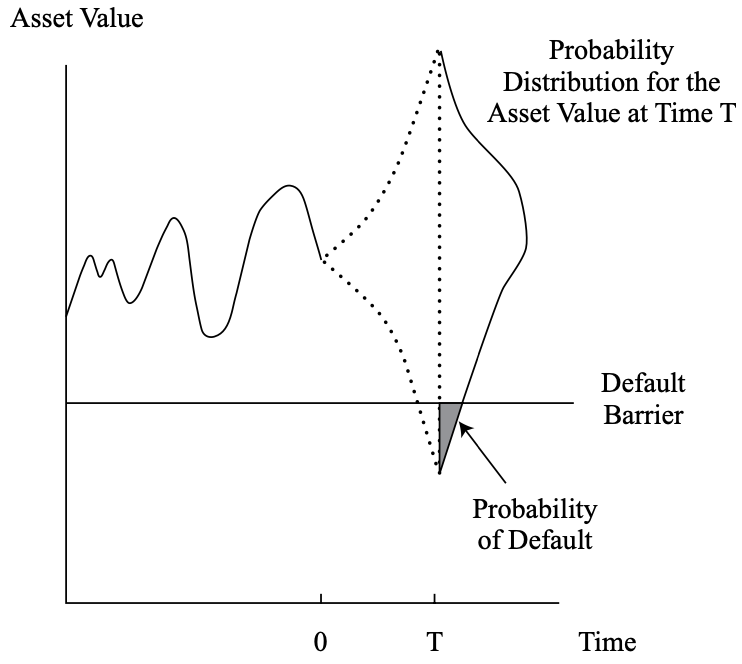
\includegraphics[scale=0.5]{/fi/structuralmodelofdefault}
\caption{Structural model of default}
\end{figure}

\begin{remark} \hlt{Structural Credit Models Interpretation of Debt and Equity as Options}\\
Let $A(T)$ be random asset value as of time $T$. Assume debt liabilities are zero-coupon bonds that mature at time $T$, with face value $K$ which is the default barrier.\\
Values for debt and equity at time $T$ are denoted $D(T)$ and $E(T)$:
\begin{align}
E(T) &= \max [A(T) - K, 0] \nonumber \\
D(T) &= A(T) - \max[A(T) - K, 0] \nonumber
\end{align}
Equity investors are long net assets and long put option, allowing them to sell assets at exercise price of $K$.\\
Risky debt investors are long position in risk-free debt and short put option (value of put  equal to CVA).
\end{remark}

\begin{remark} \hlt{Advantages of Structural Models}
\begin{enumerate}[label=\roman*.]
\setlength{\itemsep}{0pt}
\item Structural models provide an economic rationale for default, and explain why default occurs.
\item Structural models utilise option pricing models to value risky debt.
\end{enumerate}
\end{remark}

\begin{remark} \hlt{Disadvantages of Structural Models}
\begin{enumerate}[label=\roman*.]
\setlength{\itemsep}{0pt}
\item Structural models assume a simple balance sheet structure. Complex balance sheets cannot be modelled. If companies have off-balance-sheet deb, default barrier will be inaccurate.
\item Assumes assets of company are traded in the market, which is impractical.
\end{enumerate}
\end{remark}

\begin{remark} \hlt{Reduced Form Models (Intensity-Based, Stochastic Default Rate Models)}\\
Aim to explain statistically when, by modelling the default time using a Poisson stochastic process.\\
Key parameter used is default intensity (probability of default over next time increment). Estimated with regression models, includes company-specific variables and ratios, and macro-economic variables.
\end{remark}

\begin{remark} \hlt{Advantages of Reduced Form Models}
\begin{enumerate}[label=\roman*.]
\setlength{\itemsep}{0pt}
\item Model do not assume that the assets of the company trade
\item Default intensity is allowed to vary as company fundamentals and state of economy change
\end{enumerate}
\end{remark}

\begin{remark} \hlt{Disadvantages of Reduced Form Models}
\begin{enumerate}[label=\roman*.]
\setlength{\itemsep}{0pt}
\item Model do not explain why default occurs
\item Default is a random event. In reality, default is preceded by sequence of downgrades.
\item May be burdensome to implement, as modeller has to determine value of company, its volatility, default barrier based on liabilities of the company, with limitations on data availability.
\end{enumerate}
\end{remark}

\subsubsection{Valuation of Risky Bonds with Credit Spread Analysis}

\begin{method} \hlt{Bootstrapping of Discount Factor and Spot Rates with CF on Underlying Benchmark Bonds}\\
Solve for Discount Factor first,
\begin{equation}
\text{Price}_T = \sum\limits_{t=1}^T (\text{Coupon Rate}_T \times \text{DF}_t) + (\text{Price}_T \times \text{DF}_T) \nonumber
\end{equation}
Next, solve for spot rates.
\begin{equation}
\text{Spot Rate}_t = \left(\frac{1}{\text{DF}_T} \right)^{1/T} - 1 \nonumber
\end{equation}
Lastly, solve for forward rates as ratios of discount factors,
\begin{equation}
\text{Forward Rate}_{A, B-A} = \frac{\text{DF}_A}{\text{DF}_B} - 1 \nonumber
\end{equation}
\end{method}

\begin{flushleft}
\begin{tabularx}{\textwidth}{p{5em}|p{8em}|p{5em}|X|p{5em}|p{8em}}
\hline
\rowcolor{gray!30}
Maturity & Coupon Rate & Price & Discount Factor & Spot Rate & Forward Rate \\
\hline
$1$ & $-0.25\%$ & $100$ & $1.002506$ & $-0.2500\%$ & \\
$2$ & $0.75\%$ & $100$ & $0.985093$ & $0.7538\%$ & $1.7677\%$ \\
$3$ & $1.50\%$ & $100$ & $0.955848$ & $1.5166\%$ & $3.0596\%$ \\
$4$ & $2.25\%$ & $100$ & $0.913225$ & $2.2953\%$ & $4.6674\%$ \\
$5$ & $2.75\%$ & $100$ & $0.860016$ & $2.8240\%$ & $4.9664\%$ \\
\hline
\end{tabularx}
\end{flushleft}

\begin{method} \hlt{Backward Induction of Binomial Tree for Risky Bonds, Assuming No Default}\\
One-period forward rates are used, instead of spot rates. Future interest rate volatility is assumed.\\
for $t$ in range $(0, T-1, -1)$: \# Computing from second last layer to the first \\
{\color{white}space} for $n$ in layer$\_t\_$nodes:
\begin{align}
\text{v}(t,n) = \frac{\text{PMT}(t+1,n)+ [0.5 \text{v}(t+1, nH) + 0.5 \text{v}(t+1, nL)]}{1 + i(t, n)} \nonumber
\end{align}
where $\text{v}(t,n)$ is value of node at time $t$ at position $n$, $\text{v}(t+1,nH)$ and $\text{v}(t+1,nL)$ is value of node at next time step $t+1$ at positions up ($H$) and down ($L$), $\text{PMT}(t+1,n)$ is beginning coupon payment for next time step, $i(t,n)$ is interest rate at time $t$ at position $n$ in decimal. \\
Note that at last layer $T$, the value at node $n$ is as follows:
\begin{equation}
\text{v}(T, n) = \frac{\text{PMT}(T,n) + \text{Redemption Value}(T,n)}{1 + i(T, n)} \nonumber
\end{equation}
\end{method}

\begin{method} 
\label{method:computingcva}
\hlt{Computing CVA}\\
Compute expected exposure (EE) as value equal to loan or bond face value plus accrued interest, less current market value of collateral. This is typically discounted face value of bond at risk-free rate.\\
Compute recovery as Recovery Value $=$ EE $\times$ RR.\\
Compute LGD $=$ EE $\times$ $(1-$ RR$)$.\\
Compute POS $=$ $(1-$HR$)^{t-1}$.\\
Compute POD$_t$ $=$ POD $\times$ HR where HR is hazard rate.\\
Compute EL $=$ POD $\times$ LGD. \\
Compute DF$_t$ $= [1/(1+\text{Govt Bond Yield Curve Rate}_t)^t]$ \\
Compute PV EL $=$ DF $\times$ EL. Compute CVA as sum of PV EL.
\end{method}

\begin{flushleft}
\begin{tabularx}{\textwidth}{p{4em}|p{4em}|p{4em}|p{4em}|p{4em}|p{4em}|p{4em}|p{4em}|X}
\hline
\rowcolor{gray!30}
Maturity & EE & Recovery & LGD & POD & POS & EL & DF & PV EL \\
\hline
$1$ & $88.8487$ & $35.5395$ & $53.3092$ & $1.2500\%$ & $98.7500\%$ & $0.6664$ & $0.970874$ & $0.6470$ \\
$2$ & $91.5142$ & $36.6057$ & $54.9085$ & $1.2344\%$ & $97.5156\%$ & $0.6778$ & $0.942596$ & $0.6389$ \\
$3$ & $94.2596$ & $37.7038$ & $56.5558$ & $1.2189\%$ & $96.2967\%$ & $0.6894$ & $0.915142$ & $0.6309$ \\
$4$ & $97.0874$ & $38.8350$ & $58.2524$ & $1.2037\%$ & $95.0930\%$ & $0.7012$ & $0.888487$ & $0.6230$ \\
$5$ & $100.0000$ & $40.0000$ & $60.0000$ & $1.1887\%$ & $93.9043\%$ & $0.7132$ & $0.862609$ & $0.6152$ \\
& & & & $6.0957\%$ & & & CVA $=$ & $3.1549$ \\
\hline
\end{tabularx}
\end{flushleft}

\begin{method} \hlt{Valuation of Risky Bond}
\begin{enumerate}[label=\roman*.]
\setlength{\itemsep}{0pt}
\item Compute value of risky bond assuming no default (VND) based on backward induction
\begin{enumerate}[label=\arabic*.]
\setlength{\itemsep}{0pt}
\item Build binomial interest rate tree under assumption of no arbitrage
\item Apply assumption of interest rate volatility
\item Using par curve, derive implied zero-coupon rates, discount factors, forward rates
\end{enumerate}
\item Calculate credit valuation adjustment (CVA)
\begin{enumerate}[label=\arabic*.]
\setlength{\itemsep}{0pt}
\item Use risk-neutral probability of default as determined by credit model
\item Assign recovery rate based on seniority of debt issue and nature of issuer's assets
\item Calculate the present value of product of loss given default and probability of default
\end{enumerate}
\end{enumerate}
\begin{equation}
\text{Risky Bond Value} = \text{VND} - \text{CVA} \nonumber
\end{equation}
\end{method}
